%\documentclass{UUThesisTemplate}
%\begin{document}
\chapter{Motivation\label{chap2}}
At first, the terms `chiasmus', `epiphora' and `epanaphora' seem very specific to the domain of literature analysis. Do they represent any interest for other area of study? In this chapter we expose the interesting characteristics of figure of repetition that make them worth studying from a broader point of view. They present an interest in linguistics, and in computational linguistics in general as a part of artificial intelligence. We motivate why it is important to adopt an approach based on feature engineering, we then explore the range of impacts that repetitive figures have on our perception. Finally, we explain why we focus on detection. Throughout this chapter examples will be presented, most of them never presented in our articles.
\section{An Important Question for Artificial Intelligence}
As we mentioned in introduction, we are looking for \keydef{figures of speech} i.e., ``a use of language that creates a literary effect''\footnote{Definition of `rhetorical device' given by Princeton wordnet: \url{https://wordnet.princeton.edu/}} or ``an expression, [...] using words in an [...] unusual manner to add vividness, beauty, etc.'' \citep{webster1997}.
The keywords `vividness', and `beauty' cause a problem for automatic detection. These key terms belong to the lexical field of subjective human experiences which is far from the computer world. 

On the other hand we are not looking for any rhetorical figures, but just the ones that involve a repetition of words. And this part, unlike figure of speech definition, is computer friendly. We can expect that extracting the candidates is easy, thus we can dive into the artificial intelligence questions without being stopped by too important technical prerequisites.
%There is an exceptional blend between an extremely trivial definition of the basic candidates and a high cognitive experience involved by real instances of chiasmus, epiphora and epanaphora. 
This represents the ideal challenge for computational linguistics. Indeed, making the difference between an accidental repetition like \Eref{ex:analysis} and a real prototypical instance like \Eref{ex:crack} is a part of what make us humans.  
\nnumsentence{Efficiency \mn{Analysis} \mn{of} Surgical Services by Combined Use \mn{of} Data Envelopment and Gray Relational \mn{Analysis}. \label{ex:analysis}}%
%
\nnumsentence{\mn{Modeling} \mn{Cracks} and \mn{Cracking} \mn{Models}: a challenge for the future. \label{ex:crack}}%Structures, Mechanisms, Boundary Conditions, Constraints, Inconsistencies and The Proper Domains of Natural Laws.
So it is an important issue for artificial intelligence to discover what causes such distinction. %\subsection{Machine Technic}
And to discover such distinction our approach for detection will focus on hand tuned systems and machine learning. In particular, we choose to use feature engineered machine learning. There is two reasons for that. First, feature engineered systems generally need less data than deep learning systems. The biggest challenge in repetitive figure detection is to gather data and the most recent technics are very effective but designed only for big data.
Another reason why feature engineering is interesting is the self explanatory property of their models. Designing features for computers helps understanding the figures themselves and how they work.


\section{Impacts on Linguistic tasks}

Several effects can be observed in the repetitive figures. For instance, an epanaphora or an epiphora (sometimes even both of them used together as \key{symploche}) can influence the rhythm to amplify a gradation like in \Eref{ex:job}.
\nnumsentence{When you're working as an actor, you don't think that when you get out of school, it's going to be so hard to get a \mn{job}.\\
Just to get a \mn{job}.\\
Any \mn{job}. \label{ex:job}}
%
%The epiphora associated to a progressiv shrinking of the sentence accentuate the gradation in the of the meaning (from getting a job as an actor we fall progressively into getting any type of job). We observe so an example aimed at amplification of the meaning, but that is far from being the only function or rhetorical effect provoked by an epiphora or an epanaphora. 
Another use is to stress a parallelism and/or support a pun, like in \Eref{ex:bad}.
\nnumsentence{\mn{It's like} really \mn{bad}.\\
\mn{It's like} Paula-Deen-glazed-bacon-doughnut \mn{bad}. \label{ex:bad}}


%In this last example of symploche, the repetitions are important because what is stressed in these sentence is the similarity between the `really bad' and the unusual expression `Paula-Deen-glazed-bacon-doughnut bad'. Repeating the exact same words at the begining and the end of both sentences makes the sentences parallel and helps the reader understanding and accepting the neologism `Paula-Deen-glazed-bacon-doughnut'. 
If, in a linguistic task, like translation or a paraphrasing, we try to substitute the repetitions by near synonyms, we can keep the same literal meaning but the rhetorical effect vanishes instantly. In \Eref{ex:similarBad}, we observe a partial substitution of the epanaphora (`like' becomes `similar to') and in \Eref{ex:awfulBad} we practice the substitution of the epiphora by replacing the word `bad' by the word `awful' in the second sentence.
\nnumsentence{It's like really \mn{bad}.\\
It is similar to Paula-Deen-glazed-bacon-doughnut \mn{bad}.\label{ex:similarBad}}%
\nnumsentence{\mn{It's like} really bad.\\
\mn{It's like} Paula-Deen-glazed-bacon-doughnut awful. \label{ex:awfulBad}}
%It's far better to buy a {wonderful} company at a {fair} price than a {fair} company at a {wonderful} price.
None of those paraphrasing restitutes the effect of \Eref{ex:bad}. Thus the figures of repetitions have a real effect on the text and by several manners that we will only partially grab in this chapter. %and then we showed an example of paraphrase where we loose the rhetorical effect by removing the repetition. 
A second property of reptetitive figures is that they are universal as they exist in most human languages \citep{Welch1981}. And that is not without causing problems as they are sometimes, above all with chiasmus, very hard to translate (we can observe an example in English and another one in French in Examples~\ref{exGoing} and \ref{ex:sens}).%
%
\nnumsentence{When the \mn{going} gets\mn{ tough}, the \mn{tough} get \mn{going}. \label{exGoing}}%
%\nnumsentence{Nobody \mn{cares} how much you \mn{know}, until they \mn{know} how much you \mn{care}. \label{ex:care}}
\nnumsentence{Ce politicien a le \mn{sens} de la \mn{formule} qui ne \mn{formule} pas beaucoup de \mn{sens}.\footnote{This sentence criticises a politician by reverting the expression `have a way with words'/`sens de la formule'} \label{ex:sens}}%
%{Poetics} of {crisis} or {crisis} of {poetics} in digital reading/writing?
%The {paradox} of {observation} and the {observation} of {paradox}.
In these two cases a very language specific expression (`Going gets tough' and `sens de la formule') are reverted. Either you have to reproduce the chiasmus in the target language which is not always possible, either you signal the word play to the reader in a note. Anyway there can be strong difficulty of translation associated to repetitive figures and if a machine cannot perform it, at least it would be interesting if it could detect such difficulties in order to delegate this hard task to a human.
The most extreme case in which this should apply is when saving the figure of speech is even more important than saving the literal meaning. Below a real case example extracted from a movie:
\nnumsentence{Chim chiminey, chim chiminey
Chim chim cher-oo
I \mn{does} what I \mn{likes} and I \mn{likes}\ldots what I \mn{do}.\\
(Song extracted from \textit{Mary Poppins} subtitles, English version, Minute 37:18) \label{ex:song}}%
This extract is a song introducing a witty chimney sweep charachter. In the movie the use of chiasmus combined with a rhyme shows the strong literal ability of the character despite his lack of education. %signaled by the disagreement of the verbs with subjects `I'.
Now let's look at the swedish translation:%
\nnumsentence{Chim chimeney, chim chimeney
Chim chim charmer

Jag gör det jag kan
och jag kan...det jag gör\footnote{Literally `I do what I can and I can... what I do'}\\
(Song extracted from \textit{Mary Poppins} subtitles, Swedish version) \label{ex:swed}}%
The translators of this song did not preserve the literal meaning. That could be seen as a mistranslation unless we consider that in some contexts, like this song, the form prevails. The official translator prefered saving the figures of speech (rhymes combined with chiasmus) rather than the literal meaning.% What was more important in the official translator mind were the figures of speech (rhymes combined with chiasmus) rather than the literal meaning. 

\subsection{The Importance of Detection}
We saw that the importance of the rhetorical figure can go beyond the importance of the literal meaning. And we took the example of translation task. We saw as well partially the linguistic diversity of the phenomena we explore, gradation, pun, parallelism. Could there be others? There is probably much more functions existing and a mechanical detection would be a precious help for unveiling all of them. % more than translation of already well known examples or generation.

The interest of detection goes beyond the pure improvement of our linguistic knowledge. It could help classification of text. We can assume that the presence of repetitive figure is a sign of writing quality because the author took the time to create it or to quote it. Nowadays the production of texts on the web is a huge industry where authors' remuneration is often based on the number of words produced, which does not increase the quality. Thus, detecting such figures of speech is one clue (among others) that may help distinguish masterpieces from poorly written texts.

The web is not the only reason why detection has an interest. Detection answers well the  trend for \keyn{distance reading} that is raising up in literature study. \keydef{Distant reading} is the principle of ``understanding literature, not by studying particular texts, but by aggregating and analysing massive amounts of data'' \citep{Schulz2011}. %, for instance to figure out weather profession were equally distributed among men and women in the past societies.
Literature analyst could use automatic tools to detect relevant patterns that are far too rare to be observed on a massive scale with only manual reading.

Finally a last thing that pushes us to study detection more than generation is that a generator exists already for one of the most challenging repetitive figure: chiasmus.\footnote{http://tinysubversions.com/stuff/chiasmus/}
Below are 5 representative examples generated by this machine.

\nnumsentence{The \mn{spinoff} did not invent the \mn{induction}. In a very real sense, the \mn{induction} invented the \mn{spinoff}. \label{}}%
\nnumsentence{\mn{Habitats} must put an end to \mn{quarts} or \mn{quarts} will put an end to \mn{habitats}. \label{}}%
\nnumsentence{\mn{Cockpits }must put an end to\mn{ mayonnaise}s or \mn{mayonnaises} will put an end to \mn{cockpits}. \label{}}%
\nnumsentence{ Ask not what your \mn{weariness} can \mn{expel} for you, but what you can \mn{expel} for your \mn{weariness}. \label{}}%
\nnumsentence{ Ask not what your \mn{delirium} can \mn{fabricate} for you, but what you can \mn{fabricate} for your \mn{delirium}. \label{}}%
 
  We observe that the generated forms are repetitive. That is because a generator can create hundreds of examples by mimicking one or two particular pattern (here the expression `X did not invent Y. In a very real sense Y invented X', `X must put an end to Y or Y will put an end to X' and `ask not what X can Y for you, ask what you can Y for X'). When you do detection, it is not so straightforward: we will see that chiasmus for instance, and to a smaller extent epiphora and epanaphora, are rare, thus you cannot limit yourself to detect only one or two sub-patterns. We need to target a certain diversity inside the figure if we do not want to end up with a 0\% \keyn{recall}. Put this way, detection is more challenging than generation.

In this chapter we exemplified the figures and their main issues. We saw that, despite sounding like old classical terms, chiasmus, epiphora and epanaphora have the potential to help very actual challenges. The next chapter presents the historical background of the figures in rhetoric and in detection in general.
   %However, after exploring this machine and the examples generated for a while, the user realises that they always turn around the same three patterns `X did not invent Y. In a very real sense Y invented X' `X must put and end to Y or Y will put an end to X', `ask not what X can Y for you, ask what you can Y for X'. Thus the user is left with the sensation that chiasmus is a non diversified pattern which is not true. The association made by the machine is poetic, sometimes absurd (e.g., `cockpits' and `mayonnaise') but they do not look as witty as one might expect. Maybe one day machines will be able to generate witty diverse  examples, meanwhile looking for human generated examples is our best chance to catch all the diversities of the phenomenon.



%We just saw that detection will represent a challenge forcing us to grab all the diversity of the figures. We will see that we have little data on the figures. That makes the use of the most recent techniques like deep learning very difficult. Our approach will focus on feature ingeneering 
%Indeed, the phenomena we tackle are by definition rare. Thus the it is ver


%\normalsize

%In Paper~\ref{pc} we show
%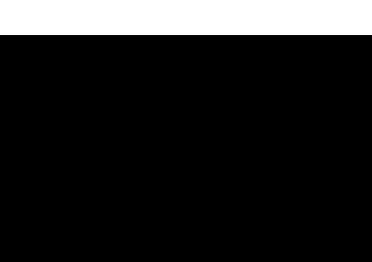
\includegraphics[scale=1]{X}
%\end{document}